\documentclass[a4paper]{article}
\usepackage{algorithmicx}
\usepackage{algpseudocode}
\usepackage{graphicx}
\usepackage{color}
\usepackage{algorithm}
\usepackage{amssymb,amsmath}
\usepackage{amsmath}
\usepackage{vmargin}
\usepackage{verbatim} % comentarios
\usepackage[utf8]{inputenc}
\usepackage{mdwlist}
\setpapersize{A4}
\setmargins{2.5cm}       % margen izquierdo
{1.5cm}                        % margen superior
{16.5cm}                      % anchura del texto
{23.42cm}                    % altura del texto
{10pt}                           % altura de los encabezados
{1cm}                           % espacio entre el texto y los encabezados
{0pt}                             % altura del pie de página
{2cm}                           % espacio entre el texto y el pie de página
\makeatletter
\setlength{\@fptop}{0pt}
\makeatother










\begin{document}

\section{Resultados}


Para los gráficos de distribución de temperaturas adoptaremos las siguientes notaciones:\newline
a: Ancho del parabrisas sin discretizar; \newline
b: Alto del parabrisas sin discretizar; \newline
h: Granularidad;\newline
n: número total de sanguijuelas;\newline
Y la temperatura en el punto crítico fue calculado con la función dameTempPtoCritico (explicada en el sección $Desarrollo$)\newline

Para el Desarrollo (creo :/):\newline

Para el experimento número uno, comportamiento de la distribucion de la temperatura, se evaluaron distintos casos. Como el cálculo de la temperatura del punto crítico difiere segun sea el tamaño del parabrisas y su posterior discretización. Se trabajó con distintos tamaños. Más aún ingresamos otros factores entre los distintos casos, como el número de sanguijuelas y  el radio de acción de cada una de estas. Además, vamos a comparar como varía la temperatura en el punto crítico (si es que lo hace) para un mismo parabrisas pero, variando la granularidad del mismo. De esta forma, aunque estamos representando a un mismo parabrisas, obtenemos discretizaciones de diferentes dimensiones.        

\subsection{Hipótesis}

Hipótesis1: A medida que la granularidad baja, la temperatura en el punto critico aumenta;\newline
Hipótesis2: Para granularidades de mayor valor las temperaturas se van distorsionando aún más;\newline
Hipótesis3: Las diferencias de temperaturas van a ser mayores si se trabaja con un parabrisas de tamaño IMPARxIMPAR;\newline
Hipótesis4: Si en un sistema predominan sanguijuelas unitarias entonces, se van a presentar mayores diferencias entre una discretización y otra.\newline


\subsection{Primer caso:}

Para el primer caso lo que se hizo fue trabajar con un parabrisas de tamaño PARxPAR (a par y b par). En el caso de la función dameTempPtoCritico ésta representacion entra como el caso IMPARxIMPAR (ya que recordemos que se resta una unidad a las medidas de ancho y alto para no contar los bordes). De esta forma, la temperatura en el punto crítico esta dada por un solo punto.
El radio de las sanguijuelas puede variar hasta los 15 metros, para tener una mayor diversidad de tamaños, y tratar de verificar lo planteado en la hipótesis5.\newline
Se trabajó con 3 discretizaciones distintas 2, 5 y 10. Los resultados se pueden observar en los gráficos: \textit{figure 1.a, figura 1.b y figure 1.c}

%140x140
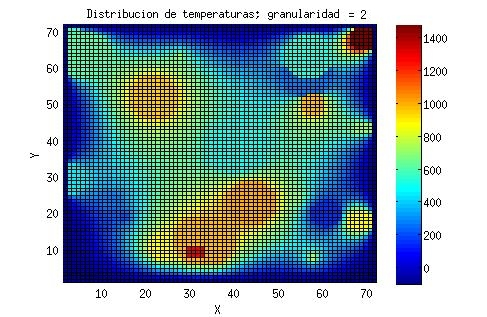
\includegraphics[width=\textwidth,height=3.0in,keepaspectratio
]{140x140h2.jpg} \newline
\begin {flushleft}
\textbf{Figure 1.a:} Distribución de temperaturas para un parabrisas con a = 140 metros; b = 140 metros; h = 2; n = 25. Donde el radio máximo de cada sanguijuela es 15 metros. Y la temperatura en el punto crítico es de 499.00000\hspace{-1.5mm}$\phantom{a}^{\circ}$c .
\end{flushleft}

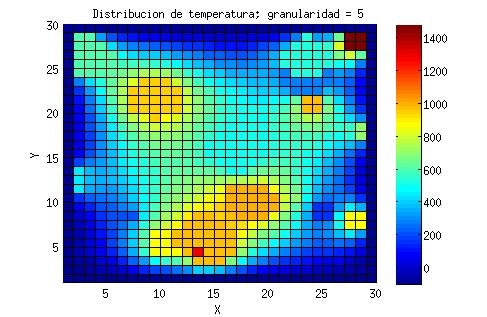
\includegraphics[width=\textwidth,height=3.0in,keepaspectratio
]{140x140h5.jpg} \newline
\begin {flushleft}
\textbf{Figure 1.b:} Mismas características que para el parabrisas representado en la $figure$ $1.a$. Pero, con granularidad igual a 5. La temperatura en el punto crítico es de 499.00000\hspace{-1.5mm}$\phantom{a}^{\circ}$c.
\end{flushleft}


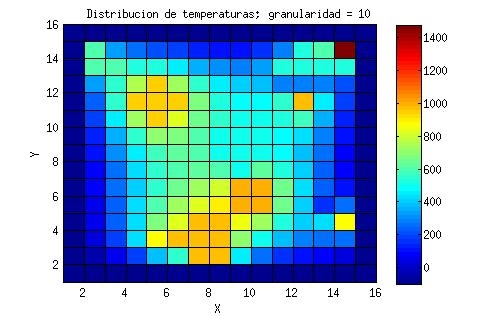
\includegraphics[width=\textwidth,height=3.0in,keepaspectratio
]{140x140h10.jpg} \newline
\begin {flushleft}
\textbf{Figure 1.c:} Mismas características que para el parabrisas representado en la $figure$ $1.a$. Pero, con granularidad igual a 10 y cuya temperatura en el punto crítico es de 499.00000\hspace{-1.5mm}$\phantom{a}^{\circ}$c .
\end{flushleft}


\subsection{Segundo caso:}


%45x45

Otro caso que analizamos fue trabajar con un parabrisas de tamaño IMPARxIMPAR (lo que se corresponde al caso PARxPAR, al momento de obtener la temperatura en el punto crítico). El mótivo de trabajar con este caso, fue que como consecuencias de las dimensiones del parabrisas la temperatura en el punto crítico ahora depende de 4 valores en total. Basta con que al menos uno de los mismos se modifique, entre las distintas discretizaciones, para que la temperatura en el punto crítico cambie. Esta idea es la que se refleja en la hipótesis3.\newline
Ademas, se trabajó con una granularidad menor a uno en este caso. Ya que a diferencia de los restantes las dimensiones del parabrisas son menores y dado que al momento de discretizar. Los parametros ancho y alto son dividos por la granularidad, el sistema cuenta con mas puntos que para los valores mayores e iguales a 1. Y para parabrisas de mayor tamaño el tiempo de computo sería excesivamente caro.  
Una caracteristica de esta experimentación es que predominan las denominadas Sanguijuelas unitarias. Dicha elección se realizo para tratar de verificar la hipótesis4. Los resultados obtenidos son los presentados en los gráficos \textit{figure 2.a, figure 2.b, figure 2.c y figure 2.d}\newline


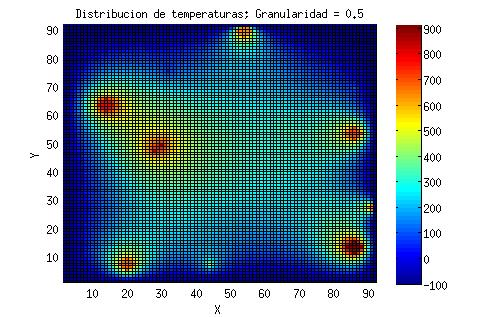
\includegraphics[width=\textwidth,height=3.0in,keepaspectratio
]{45x45h0,5.jpg} \newline
\begin {flushleft}
\textbf{Figure 2.a:} Distribución de temperaturas para un parabrisas con a = 45 metros; b = 45 metros; h = 0.5; n = 15. Donde el radio máximo de cada sanguijuela es de 2 metros. Y la temperatura en el punto crítico es de  350.69248\hspace{-1.5mm}$\phantom{a}^{\circ}$c .
\end{flushleft}

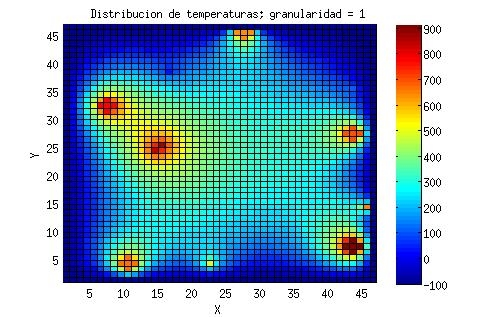
\includegraphics[width=\textwidth,height=3.0in,keepaspectratio
]{45x45h1.jpg} \newline
\begin {flushleft}
\textbf{Figure 2.b:} Mismas características que para el parabrisas representado en la $figure$ $2.a$. Pero, con granularidad igual a 5 y cuya temperatura en el punto crítico de 370.11472\hspace{-1.5mm}$\phantom{a}^{\circ}$c .
\end{flushleft}

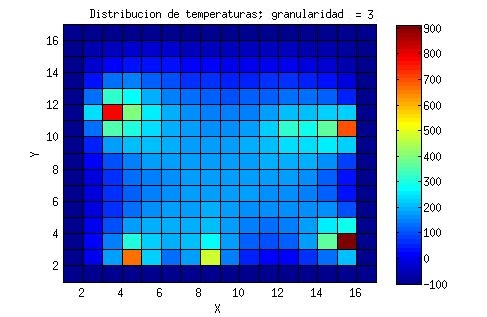
\includegraphics[width=\textwidth,height=3.0in,keepaspectratio
]{45x45h3.jpg} \newline
\begin {flushleft}
\textbf{Figure 2.c:} Se varía la granularidad del parabrisas representado por la $figure$ $2.a$ a 3. La temperatura en el punto crítico, de esta nueva representación, es de 175.58285\hspace{-1.5mm}$\phantom{a}^{\circ}$c .
\end{flushleft}

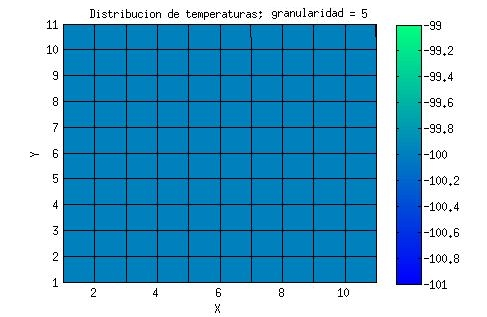
\includegraphics[width=\textwidth,height=3.0in,keepaspectratio
]{45x45h5.jpg} \newline
\begin {flushleft}
\textbf{Figure 2.d:} Mismas características que para el parabrisas representado en la $figure$ $2.a$. Pero, con granularidad igual a 5 y cuya temperatura en el punto crítico es de -100.00000\hspace{-1.5mm}$\phantom{a}^{\circ}$c.
\end{flushleft}


\subsection{Tercer caso:}


Para continuar con la idea de ver cuanto difiere las temperaturas en un parabrisas de tamaño IMPARxIMPAR. Pero, sobre todo para corroborar la hipótesis4. Se trabajó con el mismo parabrisas que en el caso anterior. Porlo que ahora se aumentó el radio de acción de las sanguijuelas de manera que haya una mayor diversidad de sanguijuelas. Ademas, que de esta forma vamos a poder conluir como afecta el radio de una sanguijuela sobre un mismo sistema. Los datos obtenidos se muestran en las figuras: \textit{figure 3.a, figure 3.b, figure 3.c}  \newline


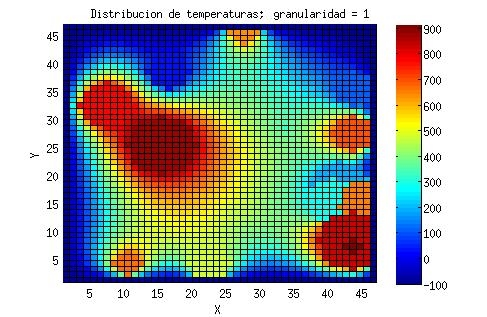
\includegraphics[width=\textwidth,height=3.0in,keepaspectratio
]{r7h1.jpg} \newline
\begin {flushleft}
\textbf{Figure 3.a:} Representación de la distribución de temperaturas para un parabrisas con a = 45 metros; b = 45 metros; h = 1; n = 15. Donde el radio máximo de cada sanguijuela es 8 metros. Y la temperatura alcanzada en el punto crítico es de 644.83827\hspace{-1.5mm}$\phantom{a}^{\circ}$c .
\end{flushleft}

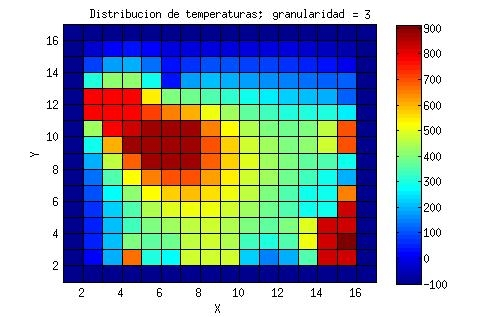
\includegraphics[width=\textwidth,height=3.0in,keepaspectratio
]{r7h3.jpg} \newline
\begin {flushleft}
\textbf{Figure 3.b:} Mismas características que para el parabrisas representado en la $figure$ $3.a$. Pero, con granularidad igual a 3. Y la temperatura alcanzada en el punto crítico es de 633.08219\hspace{-1.5mm}$\phantom{a}^{\circ}$c .
\end{flushleft}

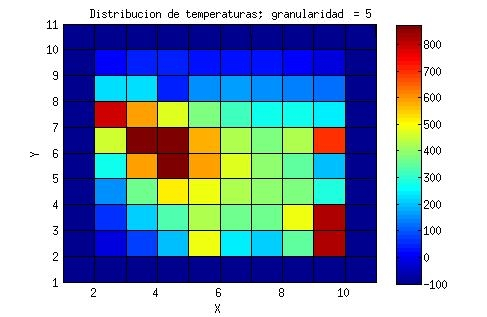
\includegraphics[width=\textwidth,height=3.0in,keepaspectratio
]{r7h5.jpg} \newline
\begin {flushleft}
\textbf{Figure 3.c:} Mismas características que para el parabrisas representado en la $figure$ $3.a$. Pero, con granularidad igual a 5 y cuya temperatura en el punto crítico es igual a 515.79566\hspace{-1.5mm}$\phantom{a}^{\circ}$c .
\end{flushleft}


\subsection{Cuarto caso:}


Debido a que en los anteriores caso el valor del punto crítico dependia de uno o cuatro valores. Se decidió ver la última variante que existe, que es cuando un parabrisas tiene un lado par y el otro impar. De esta forma, el punto crítico depende del promedio entre dos valores. \newline
Este caso nos resulta útil para tratar de corroborar la veracidad de la hipótesis3. Para acercanos a un caso promedio en el que no solo van a aparecer sanguijuelas con radio acción bajo, el mismo puede variar hasta los 10 metros. Los gráficos presentados a continuación reflejan los datos obtenidos.    

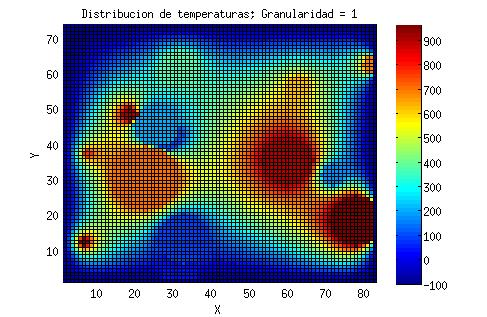
\includegraphics[width=\textwidth,height=3.0in,keepaspectratio
]{82x71h1.jpg} \newline
\begin {flushleft}
\textbf{Figure 4.a:} Representación de la distribución de temperaturas para un parabrisas con a = 81 metros; b = 71 metros; h = 1; n = 15. Donde el radio máximo de cada sanguijuela es de 10 metros. La temperatura en el punto crítico es de 533.86579\hspace{-1.5mm}$\phantom{a}^{\circ}$c .
\end{flushleft}

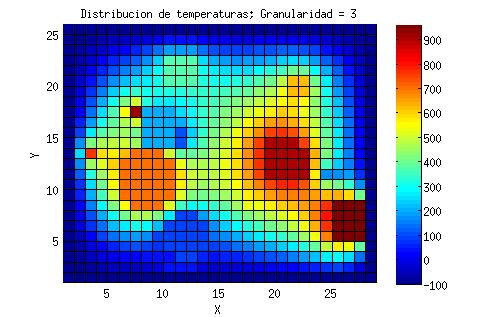
\includegraphics[width=\textwidth,height=3.0in,keepaspectratio
]{82x71h3.jpg} \newline
\begin {flushleft}
\textbf{Figure 4.b:} Mismas características que para el parabrisas representado en la $figure$ $4.a$. Pero, con granularidad igual a 3. Y la temperatura alcanzada en el punto crítico es de 495.18948\hspace{-1.5mm}$\phantom{a}^{\circ}$c .
\end{flushleft}

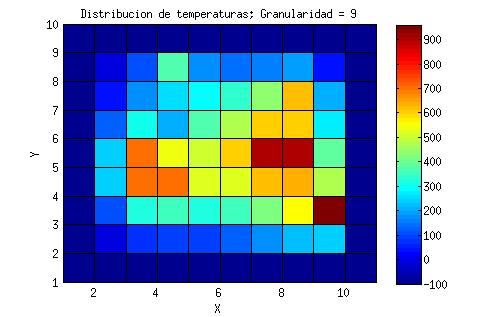
\includegraphics[width=\textwidth,height=3.0in,keepaspectratio
]{82x71h9.jpg} \newline
\begin {flushleft}
\textbf{Figure 4.c:} Mismas características que para el parabrisas representado en la $figure$ $4.a$. Pero, con granularidad igual a 5 y cuya temperatura en el punto crítico es de 552.85704\hspace{-1.5mm}$\phantom{a}^{\circ}$c .
\end{flushleft}


\section{Discusiones:}


Hipótesis1: Apartir de los experimentos realizados podemos concluir que la Hipótesis1 es falsa. Debido a diversos mótivos. En el caso número 1, variamos notablemente el valor de las granuladidades con las cuales trabajamos, yendo desde el valor 2 hasta el 10. Y en todos los casos obtuvimos la misma temperatura en el punto crítico. Ademas como se puede observar en \textit{figure 1.a, figure 1.b y figure 1.c}, los puntos restantes poseen una distribución de temperaturas muy similar entre cada Gráfico. En este caso, la temperatura en el punto critico se mantuvo constante entre cada representación.
En el caso número 2, se varío la granuladidad y los valores se modificaron (si bien representa un caso particular, donde las sanguijuelas son mayormente unitarias. sigue siendo un caso posible). Podemos observar que el valor del punto critico en la $figure$ $2.d$ es menor que en la de $2.c$, la cual es menor a su vez que en la obtenida en la $figure$ $2.b$  (entre cada gráfico fuimos disminuyendo el valor de la granularidad). Sin embargo, cuando probamos con h = 0.5, la temperatura en el punto crítico para este caso fue de 350.69248\hspace{-1.5mm}$\phantom{a}^{\circ}$c (ver $figure$ $2.a$) siendo menor que la obtenida para una granularidad de valor 1 ($figure$ $2.b$). Falseando nuestra hipótesis. \newline
El origen de pensar en esta hipótesis se basó en la idea de que al discretizar el sistema por valores de h mas grandes obtenemos menos puntos y la distancia entre ellos es mayor. Asi, si entre dos puntos $A_{ij}$, $A_{i+1,j}$ (de un parabrisas A, discretizado), existía una distancia de valor $h'$ (valor de la granularidad). Y una sanguijuela actua sobre la posicion $i'$ $j'$ con radio $r$ (en el parabrisas sin discretizar) con $j$ $=$ $h'*j'$ e $i*h'$ $<$ $i'$ $+$ $r$ $<$ $(i+1)*h'$. Entonces esa sanguijuela se omitiria (ya que no afecta a ningún punto de la discretización) obteniendo un sistema con una sanguijuela menos y por lo tanto un punto de calor menos. Que si se trabajase con un $h''$, $h''$ $<$ $h'$ e $i'*h''$ $>=$ $i'*r$ $\vee$ $i'*h''$ $<=$ $i'$ $+$ $r$. Al observar este comportamiento ahora fue necesario analizar el por qué de este hecho (agregar si ya hicieron este caso sino explicar).\newline \newline

Hipótesis2: Si bien apartir del experimento anterior podemos ver que no se cumple dicha hipótesis. No podemos dar por totalmente erronea a la misma. Sino, que llegamos a la conclusión de que depende el caso con el que se trabaje. Ya que a diferencia del caso 1. En los otros gráficos (PAGINAS LAS QUE QUEDEN) se puede observar que varían las temperaturas para distintas granularidades. Aún más en la figure 2.d se detalla que el punto crítico (y se puede observar) tiene una temperatura de -100\hspace{-1.5mm}$\phantom{a}^{\circ}$c mientras que para el mismo sistema pero con otra discretizacion alcanza una temperatura de  350.69248\hspace{-1.5mm}$\phantom{a}^{\circ}$c (ver $figure$ $2.a$ ). Siendo la mayor diferencia de temperatura que se registró entre los distintos casos (el por qué de este hecho lo desarrollaremos a lo largo de la hipótesis3 e hipótesis4). Dado que él único caso en el que no se produce un cambio en las temperaturas es el uno. Podemos concluir que se debe a las características propias que presenta el primer caso y que los restantes no. Como tratarse de sistema con sanguijuelas de distintos tamaños. También ser de la forma PARxPAR. Ya que de esta forma el punto crítico solo depende un solo punto de la discretización y es el central. Por lo que si hay una sanguijuela, cuyo radio afecta en este punto y es lo sufientemente grande para permanecer con las granularidades que se utilicen entonces siempre vamos a obtener la misma temperatura en el punto crítico. \newline \newline


Hipótesis3: Trabajamos con una parabrisas de forma IMPARxIMPAR en las PAGINAS LAS QUE SEAN, (segundo y tercer caso del experimento número uno) Por hipóstesis, estos deberian ser los casos donde la temperatura del punto crítico varíe mas entre cada discretizacion utilizada. Y para el primer caso lo es, como ya se menciono se en este sistema se presentó la mayor diferencia. Sin embargo, para el mismo sistema con sanguijuelas de radio mayor (vease caso PAG) la temperatura cambió pero, no tan bruscamente, de hecho en porcentaje es muy similar al caso número 4 (pag). Donde las temperaturas en el punto crítico y en el resto, como puede verse, se mantienen muy similares. Entonces hay otro factor que influye además de que la matriz sea IMPARxIMPAR. Por lo que la hipótesis se podría mejorar diciendo que si se trabaja con una matrix IMPARxIMPAR o un lado PAR y el otro IMPAR (y sanguijuelas de radio variado, hecho analizado en la hipótesis 4). Se van a obtener mayores diferencias que utilizando otras dimensiones con sanguijuelas de radio variado.\newline \newline


Hipótesis4: Como ya hicimos referencia anteriormente los cambios de temperatura más notable se presentaron en el caso 2 (PAG). Y fue donde trabajamos con un predominio de sanguijuelas unitarias. Este cambio no solo se nota en el punto crítico sino que como se puede ver entre la $figure$ $2.a$ y la $figure$ $2.c$ varias puntos afectados por sanguijuelas se pierden entre cada experimentación, aquellos con temperaturas no mayor a los 400\hspace{-1.5mm}$\phantom{a}^{\circ}$c, se pierden en la siguiente experimentacion. Solo permanecen aquellos en los que el radio de accion es mayor a 0. Luego en la $figura$ $2.d$ se perdieron todos los puntos sobre los cuales actuaban las sanguijuelas. De esta forma, y pese a que la granularidad no varío tanto entre los distintos experimentos; Como por ejemplo entre la $figure$ $4.a$ y la $figure$ $4.d$ donde la granularidad va de 1 a 9 o  incluso el mismo sistema pero  con sanguijuelas de mayor tamaño caso 3 (PAG). Podemos concluir que la hipotesis (para estos casos) es verdadera. Más aún, podemos concluir en general que variar las granularidades puede llegar a afectar el resultado de la distribucion de las temperaturas, según el tipo de dimensiones del parabrisas. Pero, que este no es el único factor de distorsión, sino que también esta dado por el radio de las sanguijuelas, afectando en mayor medida si el mismo es de tamaño muy bajo.  




\section{Desarrollo:}


Uno de los objetivos del presente trabajo es determinar si se puede salvar el parabrisas eliminando una sola sanguijuela. Y de ser posible que eliminemos la mejor. Para esto se plantean dos posibles formas. La segunda es utilizar la fórmula Sherman–Morrison* (CITAR FUENTE CON LA EXPLICACION) la misma plantea que:

\begin{equation}
	(A+ uv^t)^{-1} \ =\ A^{-1} - \frac{ A^{-1} u v^t A^{-1} }{1+v^t A^{-1}u}.\label{eq:sm}
\end{equation} 
\textit{Siendo A una matriz inversible, y u, $v^t$ dos vectores.}


Aplicandola siempre que sea posible su uso. Para esto analicemos el caso de un sistema que posee al menos una sanguijuela unitaria, luego de discretizar y platear el sistema de ecuaciones para el problema obtendremos una matriz como la siguiente:

$$
A_{n,n} =
 \begin{pmatrix}
  4_{1,1} & -1_{1,2} & \cdots & -1_{1,1+t} & \cdots & \cdots & \cdots & \cdots  & 0_{1,n} | & -200 \\
   -1_{2,1} & 4_{2,2} & -1_{2,3} & \cdots -1_{1,2+t} & \cdots & \cdots & \cdots & \cdots & 0_{2,n} | & -100 \\
  \vdots  & \vdots  & \vdots & \vdots  & \ddots & \vdots  & \vdots & \vdots & \vdots\\
  \vdots  & \vdots & \vdots & \vdots  & \ddots & \vdots  & \vdots & \vdots & \vdots\\
   0_{i,1} & 0_{i,i-t} & \cdots & 0_{i,i-1} & 1_{i,i} &  0_{i,i+1} & \cdots & 0_{i,i+t} & \cdots | & T_{sang_i} \\
  \vdots  & \vdots  & \vdots & \vdots  & \ddots  & \vdots  & \vdots & \vdots & \vdots\\
  \vdots  & \vdots  & \vdots & \vdots  & \ddots  & \vdots  & \vdots & \vdots & \vdots\\
   0_{n-1,1} & \cdots & \cdots & \cdots & -1_{n-1,n-1-t} & \cdots & -1_{n-1,n-2} & 4_{n-1,n-1} &  -1_{n-1,n} | & -100 \\
   0_{n,1} & \cdots & \cdots & \cdots & \cdots & -1_{n,n-t} & \cdots & -1_{n,n-1} &  4_{n,n} | & -200 \\
 \end{pmatrix}
$$
\textit{la fila i, representa a la sanguijuela unitaria $sang_i$, con $T_{sang_i}$ su correspondiente temperatura y con las coordenadas (x,y) en la discretizacion.}\newline

Con el sistema a resolver Ax = b.\newline
Pero, al eliminar $sang_i$ ese punto dejara de tener el valor $T_{Sang_i}$. Para pasar a ser el promedio de los puntos (x+1,y), (x-1,y), (x,y+ancho), (x, y-ancho)(con ancho referenciamos al ancho del parabrisas discretizado y sin contar los bordes). De esta forma obtenemos el siguiente sistema: A'x = b'.\newline Con la matriz asociada:

$$
A'_{n,n} =
 \begin{pmatrix}
  4_{1,1} & -1_{1,2} & \cdots & -1_{1,1+t} & \cdots & \cdots & \cdots & \cdots  & 0_{1,n} | & -200 \\
   -1_{2,1} & 4_{2,2} & -1_{2,3} & \cdots -1_{1,2+t} & \cdots & \cdots & \cdots & \cdots & 0_{2,n} | & -100 \\
  \vdots  & \vdots  & \vdots & \vdots  & \ddots & \vdots  & \vdots & \vdots & \vdots\\
  \vdots  & \vdots & \vdots & \vdots  & \ddots & \vdots  & \vdots & \vdots & \vdots\\
   0_{i,1} & -1_{i,i-t} & \cdots & -1_{i,i-1} & 4_{i,i} &  -1_{i,i+1} & \cdots & -1_{i,i+t} & \cdots | & 0 \\
  \vdots  & \vdots  & \vdots & \vdots  & \ddots  & \vdots  & \vdots & \vdots & \vdots\\
  \vdots  & \vdots  & \vdots & \vdots  & \ddots  & \vdots  & \vdots & \vdots & \vdots\\
   0_{n-1,1} & \cdots & \cdots & \cdots & -1_{n-1,n-1-t} & \cdots & -1_{n-1,n-2} & 4_{n-1,n-1} &  -1_{n-1,n} | & -100 \\
   0_{n,1} & \cdots & \cdots & \cdots & \cdots & -1_{n,n-t} & \cdots & -1_{n,n-1} &  4_{n,n} | & -200 \\
 \end{pmatrix}
$$


Notemos que la única modificacion se produjo en la fila i. El resto de la matriz sigue siendo la misma. Entonces podriamos reescribir a A' como:

A' = A + B (1);\newline
Para algun B conveniente\newline
Por lo que 
B = A' - A \newline

Denotemos a cada matriz de la siguiente forma:\newline
$$
A=
\begin{pmatrix} 
A_1^t\\
A_2^t\\
.\\
.\\
A_i^t\\
.\\
.\\
A_n^t
\end{pmatrix}
\quad
;A'=
\begin{pmatrix} 
$A'$_1^t\\
$A'$_2^t\\
.\\
.\\
$A'$_i^t\\
.\\
.\\
$A'$_n^t
\end{pmatrix}
\quad
;B = A - A' =
\begin{pmatrix} 
A_1^t - $A'$_1^t \\
A_2^t - $A'$_2^t \\
.\\
.\\
A_i^t - $A'$_i^t \\
.\\
.\\
A_n^t - $A'$_n^t 
\end{pmatrix}
(2)
$$

$con$ $A_j$, $B_j$, $A'_j$ $\in$ $\Re^n$, $\forall$ j, 1 $<=$ j $<=$ n\newline

Como ya dijimos $\forall$ j, j $\neq$ i, $A_j$ $=$ $A'_j$
Entonces a partir de (2) podemos concluir que $\forall$ j, j $\neq$ i, $B_j = 0$\newline

Mientras que:\newline
$B_i$ $=$ $A'_i$ - $A_i$\newline  
$B_i$ =  $(0,..,-1_{i,i-a},..,-1,4_{i,i},-1,..,-1_{i,i+a}..,0)$ - $(0,...0,1_{i,i},0,...,0)$\newline
$B_i$ = $(0,..,-1_{i,i-a},..,-1,3_{i,i},-1,..,-1_{i,i+a}..,0)$. (Siendo a el ancho del parabrisas discretizado)\newline

De esta manera ya conocemos nuestra matriz B. dado que B $\in$ $\Re^{nxn}$. Podemos pensar a B como el producto de dos vectores u y $v^t$, con u,v $\in$ $\Re^{n}$
  

1) Primero empezemos por analizar el producto en general de estos dos vectores: 
$$
u=
\begin{pmatrix} 
u_1\\
u_2\\
.\\
.\\
u_i\\
.\\
.\\
u_n
\end{pmatrix}
\quad
 ;v^t=
\begin{pmatrix} 
v_1,...,v_2,...v_n
\end{pmatrix}
\quad
;u*v^t=
\begin{pmatrix} 
u_1*v_1 \cdots u_1*v_k \cdots u_1*v_n\\
u_2*v_1 \cdots u_2*v_k  \cdots u_2*v_n\\
.\\
.\\
u_i*v_1 \cdots u_i*v_k \cdots u_i*v_n\\
.\\
.\\
u_n*v_1 \cdots u_n*v_k  \cdots u_n*v_n
\end{pmatrix}
\quad
=
\begin{pmatrix} 
u_1*v^t\\
u_2*v^t\\
.\\
.\\
u_i*v^t\\
.\\
.\\
u_n*v^t
\end{pmatrix}
$$

Como queremos que B = $u*v^t$
$$
\begin{pmatrix} 
0\\
0\\
.\\
.\\
B_i\\
.\\
.\\
0
\end{pmatrix}
\quad
=
\begin{pmatrix} 
u_1*v^t\\
u_2*v^t\\
.\\
.\\
u_i*v^t\\
.\\
.\\
u_n*v^t
\end{pmatrix}
$$

Por lo que si pensamos a u como el vector canónico $e_i$ y a $v^t$ como la fila que queremos sumar, es decir como $B_i$ tenemos que:


$$
u*v^t=
\begin{pmatrix} 
0*B_i\\
0*B_i\\
.\\
.\\
1*B_i\\
.\\
.\\
0*B_i
\end{pmatrix}
\quad 
=
\begin{pmatrix} 
0\\
0\\
.\\
.\\
B_i\\
.\\
.\\
0
\end{pmatrix}
$$

El objetivo es resolver:\newline
A'x = b'\newline 
(A + B)x = b' por (1) \newline
(A + u$v^t$)x  = b'\newline
Como A' es inversible
$(A + u*v^t)^{-1}b'$ = x\newline
Pero ahora podemos aplicar la formula de Sherman–Morrison, de esta manera tenemos que: 

\begin{equation}
x =\ A^{-1}*b' - \frac{ A^{-1} u v^t A^{-1}*b'}{1+v^t A^{-1}u}.\label{eq:sm}(3)
\end{equation} 

De esta fórmula lo único que resta calcular es: $A^{-1}$*u (4) y $A^{-1}*b'$ (5).\newline
Pero, podemos reescribir a (4) y a (5) como:\newline
 A*z = u y A*y = b'. Y resolver ambos sistemas. Pudiendo concluir que la fórmula es aplicable cada vez que queremos eliminar una sanguijuela unitaria. \newline
 
 
\textbf{Análisis de la complejidad y algoritmo:} \newline

A continuación se presenta un pseudo-código del algoritmo implementado para la fórmula Sherman–Morrison:

 \begin{algorithm}[H]
\caption{Sherman–Morrison(matriz L, matriz U, vector u, coordenadas (x,y))}
\begin{algorithmic}[1]

\State $ z' \gets ForWardSubstitution(u, L)$ O($n^2$)
\State $ A^{-1}*u \gets BackWardSubstitution(z', U)$ O($n^2$)
\State $ y \gets ForWardSubstitution(b', L)$ O($n^2$)
\State $ A^{-1}*b' \gets BackWardSubstitution(y, U)$ O($n^2$)
\State $ v^t \gets$ $vector$ $de$ $longitud$ $5$ (*1) O(1)
	\If {(\textit{x no esta en el borde superior})}
        		\State $ v^t[1] \gets -1  $	O(1)	
	\EndIf
	\If {(\textit{x no esta en el borde derecho})}
        		\State $ v^t[2] \gets -1  $ 	O(1)	
	\EndIf
			\State $ v^t[3] \gets 3  $ O(1)
	\If {(\textit{x no esta en el borde izquierdo})}
        		\State $ v^t[4] \gets -1  $ 	O(1)	
	\EndIf
	\If {(\textit{x no esta en el borde inferior})}
        		\State $ v^t[5] \gets -1  $ 	O(1)	
	\EndIf
	(En los casos contrarios completar la posición de $v^t$ con cero) O(1)
	 \State $ k \gets 0  $ 	O(1)
	 \State $ l \gets 1  $   O(1)
\For{i = 1 to 5 }	
	\If {(\textit{$v^t[i]$ != 0})}
        		\State k $\gets$ \textit{(producto de $v^t[i]$ con $ A^{-1}*b'$ segun la fila a la cual hace referencia)} + k;	(*2)	 O(1)*5
        		\State l $\gets$ \textit{(producto de $v^t[i]$ con $A^{-1}*u$ segun la fila a la cual hace referencia)} + l; O(1)*5
	\EndIf
\EndFor
\State  Return \textit{devolver un vector con las restas entre  $(A^{-1}*b)[i]$ y  $((k/l)A^{-1}*u)[i]$}    O(n)

\end{algorithmic}
\end{algorithm}
\textit{Siendo L y U las correspondientes matrices de la factorizaci\'on LU de A; u es el vector can\'onico $e_i$, con i la fila que representa en la matriz la sanguijuela a eliminar; y las coordenadas (x,y) del parabrisas discretizado (recordemos que en el parabrisas discretizado no contamos los bordes del parabrisas original. Por lo que al referirnos a bordes en el pseudo-c\'odigo hacemos referencia a la nueva representaci\'on)}\newline\newline
 \textbf{Explicación:}\newline  
Empezando por las operaciones A*z = u y A*y = b': \newline
Si ya contamos con la factorización LU de A, reescribimos:\newline
LU*z = u; \newline
llamamos z' = U*z (6) y L*z' = u (7);\newline
Resolvemos (7) mediante la técnica Forward Substitution. Y realizado esto, podemos calcular (6) aplicando Backward Substitución. De esta forma la complejidad de ambas técnicas cuestan O($n^2$). Siguiendo la misma idea resolvemos 
A*y = b' en O($n^2$). Luego, procedemos a efectuar los productos $v^t A^{-1}*b'$ (8)y $v^t A^{-1}u$ (9). En (*1) se crea el vector $v^t$ pero con un tamaño igual a 5, ya que como se explico en la PAG el mismo  se utiliza como la nueva fila que hay que sumarle a A para llegar a A'. Por lo que su tamaño debería ser igual al largo de la fila de ambas matrices. Sin embargo, como a lo sumo solo va a poseer 5 valores distintos de cero, optamos por acotar su tamaño. Siguiendo con el producto (8), en (*2) efectuamos esta operación. Teniendo en cuenta la idea del vector $v^t$, $v^t$[1] se corresponde con la posición f - ancho del vector solución de $A^{-1}*b'$ (f fila en la que se representan las coordenadas(x,y) en la matriz asociada al parabrisas discretizado. La misma fue calculada como f = ancho*y + x); $v^t$[2] con f-1 de dicho vector, etc. De esta manera obtenemos el escalar solución en O(1). Con la misma logica obtenemos el escalar $1+v^t A^{-1}u$ en O(1). Lo que resta hacer es la diferencia entre ambos vectores soluciones (linea 27), costo O(n). Por lo que el costo temporal total, para eliminar k sanguijuelas unitarias, es k.O($n^2$) + O($n^3$) (costo de obtener LU).\newline\newline

\textbf{Matriz LU y bandas:}

Consideremos A una matriz banda, A $\in$ $\Re^{nxn}$, con $b_s$ y $b_i$ las bandas superiores e inferiores correspondientemente y $b_s$ $=$ d, $b_i$ $=$ d.\newline
Al momento de representar la matriz LU de A, se aprovechó que la misma fuese bandas. Ya que entonces, la matriz LU hereda el número de bandas de A. Para la matriz L, esto se puede ver al momento de aplicar la Eliminación Gaussiana en una matriz de este tipo. Si desarrollamos el primer paso de la eliminacion Gaussaiana lo que se  realiza es la diferencia entre $F_i$ - $(a_{1,1}/a_{i,1})1*F_1$, $\forall$ $2 <= i <= d+1$. Notemos que i solo tiene que llegar hasta $d+1$ debido a que se trata de una matriz banda (el por qué de este hecho se explicó en la pág). A su vez, en el primer paso podemos obtener los multiplicando:  \{$l_{2,1}$= $a_{1,1}/a_{2,1}$, $l_{3,1}$ = $a_{1,1}/a_{3,1}$, . . .,$l_{d+1,1}$ = $a_{1,1}/a_{d+1,1}$,\}; en el siguiente paso haremos  $F_i$ - $(a_{2,2}/a_{i,2})1*F_2$, $\forall$ $3 <= i <= d+2$ y obtendremos: \{$l_{3,2}$ $=$ $a_{2,2}/a_{3,2}$, $l_{4,1}$ $=$ $a_{2,2}/a_{4,2}$, . . . $l_{d+2,2}$ $=$ $a_{2,2}/a_{d+2,2}$,\}, así hasta calcular $F_{n-1}$ - $(a_{n-1,n-1}/a_{n,n-1})1*F_{n-1}$ y obteniendo el multiplicando $l_{n,n-1}$ = $(a_{n-1,n-1}/a_{n,n-1})$.  Notemos los últimos multiplicando de cada paso, y obtenemos: \{$l_{d+1,1}$, $l_{d+2,2}$, . . ,$l_{d+i,i}$, . . ,$l_{n,n-1}$,\}. Es decir que los elementos de las filas $fila_i$ $d+2<= i <= n$ son ceros hasta la columna i, lo cual es el comportamiento de una matriz banda con $b_i$ = d. Si lo representamos obtenemos la matriz L = 

$$
 \begin{pmatrix}
    1 \\
  l_{2,1} & 1\\
  l_{3,1} & l_{3,2} & 1 \\
  \vdots  & \vdots  & \vdots &  \\
   l_{d+1,1} & l_{d+1, 2} & \cdots & l_{d+1,d} & 1 \\
   0 & l_{d+2, 2} & l_{d+2, 3} & \cdots &l_{d+2,d+1} & 1\\
  \vdots  & \ddots  & &  &  & \vdots  &  \\
  \vdots  &  & 0 & l_{n-1,n-1-d} & \cdots & \cdots & l_{n-1,n-2} & 1 \\
  0 & \cdots & \cdots & 0 & l_{n,n-1-d} & \cdots & \cdots & \cdots & l_{n,n-1} & 1

  
 \end{pmatrix}
$$
\textit{representaci\'on de los elementos ubicados antes de la diagonal, quienes conforman la matriz L. }\newline
Como se puede observar la matriz L tiene d bandas inferiores, al igual que la matriz A. \newline \newline


Mientras que para la matriz U, si $d_s$ $=$ d significa que heredó la misma cantidad de ceros que no conformaban las bandas superiores del triangulante superior. Esto se observa cuando realizamos las restas entre filas en la Eliminación Gaussiana tomemos el paso k. La misma establece que debemos realizar $F_i$ $-$ $(a_{i,k}/a_{k,k})*F_k$, $\forall$ $k+1<= i <= min(n,k+d)$. como A tiene d bandas superiores, luego de la posición $a_{k,k+d}$ la $fila_k$ tiene ceros. Cuando se realiza $F_i$ $-$ $(a_{i,k}/a_{k,k})*F_k$, luego de $a_{i,i+d}$ $F_i$ tiene ceros y como k+d $<$i+d. Todas las posiciones luego de i+d van a seguir siendo cero ya que se estan restando solo estos valores. Es por esto que en la Eliminacion Gaussiana implementada, cuando calculamos la diferencia entre dos fila sólo lo hacemos entre d de sus elementos.       \newline \newline

Al conocer las propiedades que va a tener la matriz LU (la misma cantidad de bandas que la matriz a la cual se aplicó dicha factorización). Para optimizar en costo espacial. Lo que se implementó fue, que a medidad que se factorizaba la matriz A guardabamos los multiplicando en la misma matriz. Y luego, mediante dos funciones, pedir la matriz L y la matriz U. Cada una respresentada con un vector de vectores. Pero, como cada fila de las mismas tiene a lo sumo d+1 elementos distintos de cero (con d la cantidad de bandas superiores e inferiores y el uno que se adiciona es por contar el elemento de la diagonal) cada uno de los vectores interiores era de a lo sumo de tamaño d+1. Representando de esta manera solo los elementos que se ubican dentro de las bandas correspondientes para cada matriz.     





\end{document}